% Autor: Daniel Tatzel

\section{Suchfunktion}

\subsection{Autovervollständigung}

Im Layout auf der rechten Seite integriert, findet man die globale Suchfunktion der Webseite. 
Sobald ein Nutzer zwei oder mehr Zeichen eingibt, wird in der Datenbank nach 
möglichen Treffern zu der Eingabe gesucht, und dem Nutzer werden Vorschläge zur Vervollständigung seiner Eingabe dargestellt.
\begin{figure}[!htbp]
\centering
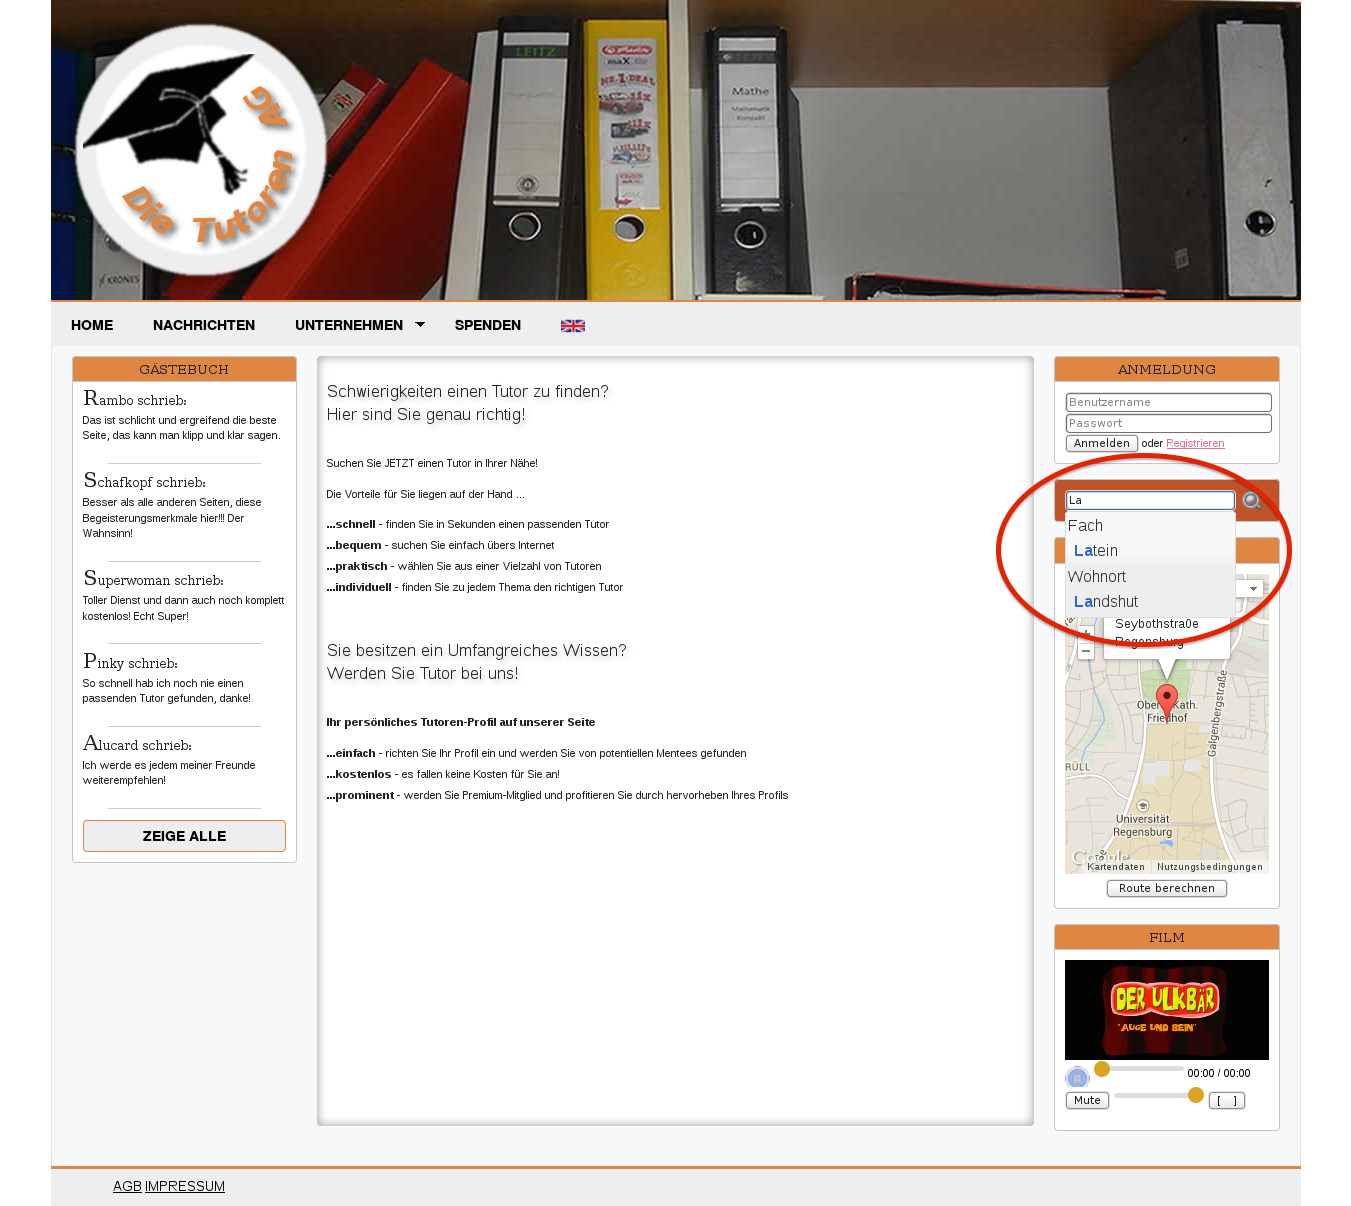
\includegraphics[width=1\linewidth]{../Screenshots/de/Autocompletion}
\caption{Autovervollständigung}
\label{fig:Autovervollstaendigung}
\end{figure}

\newpage
\subsection{Suche nach Fächern}

Wird von der Suchfunktion erkannt, das nach einem Fach gesucht wird, erhält der 
Nutzer eine spezielle Seite mit Tutoren welche das gesuchte Fach unterrichten. 
Somit spart sich der Nutzer Zeit, und wird direkt auf die richtige Seite 
weitergeleitet, anstatt Ihm die Standard Suchergebnisse zu zeigen.
\begin{figure}[!htbp]
\centering
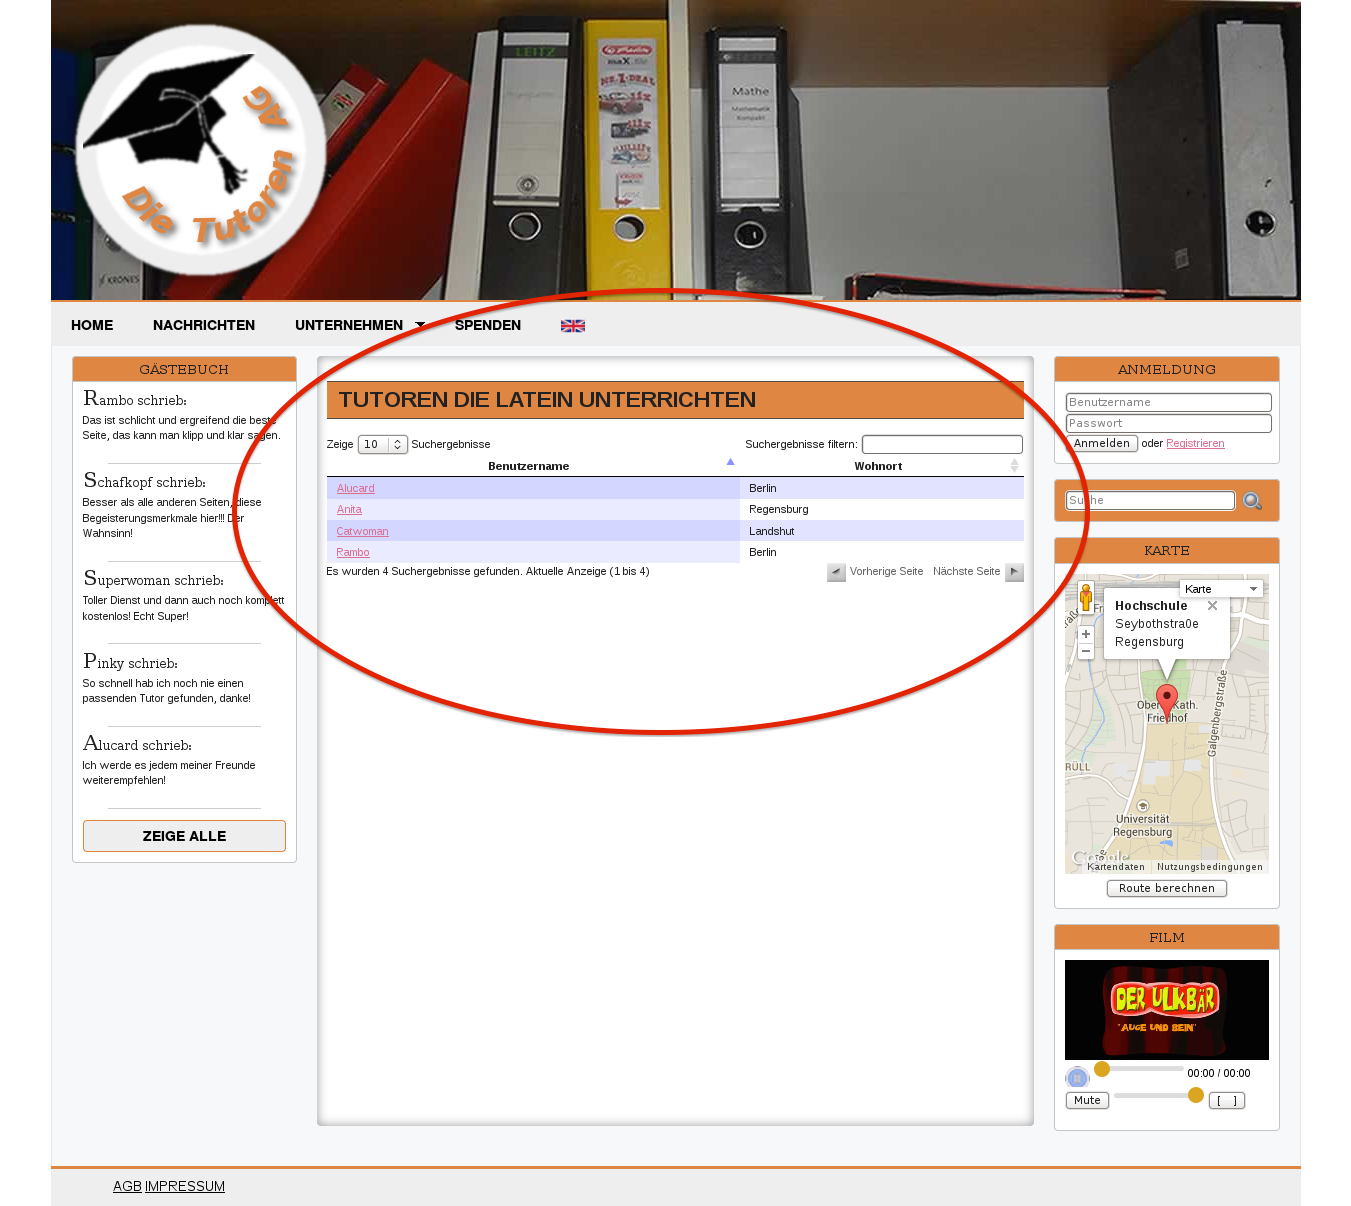
\includegraphics[width=1\linewidth]{../Screenshots/de/Suche_Fach}
\caption{Suchausgabe Fach}
\label{fig:SuchausgabeFach}
\end{figure}


\newpage

\subsection{Suche nach Wohnorten}

Wird von der Suchfunktion erkannt, das nach einem Ort gesucht wird, erhält der 
Nutzer eine spezielle Seite mit Tutoren welche an dem gesuchten Ort unterrichten. 
Somit spart sich der Nutzer Zeit, und wird direkt auf die richtige Seite 
weitergeleitet, anstatt Ihm die Standard Suchergebnisse zu zeigen.
\begin{figure}[!htbp]
\centering
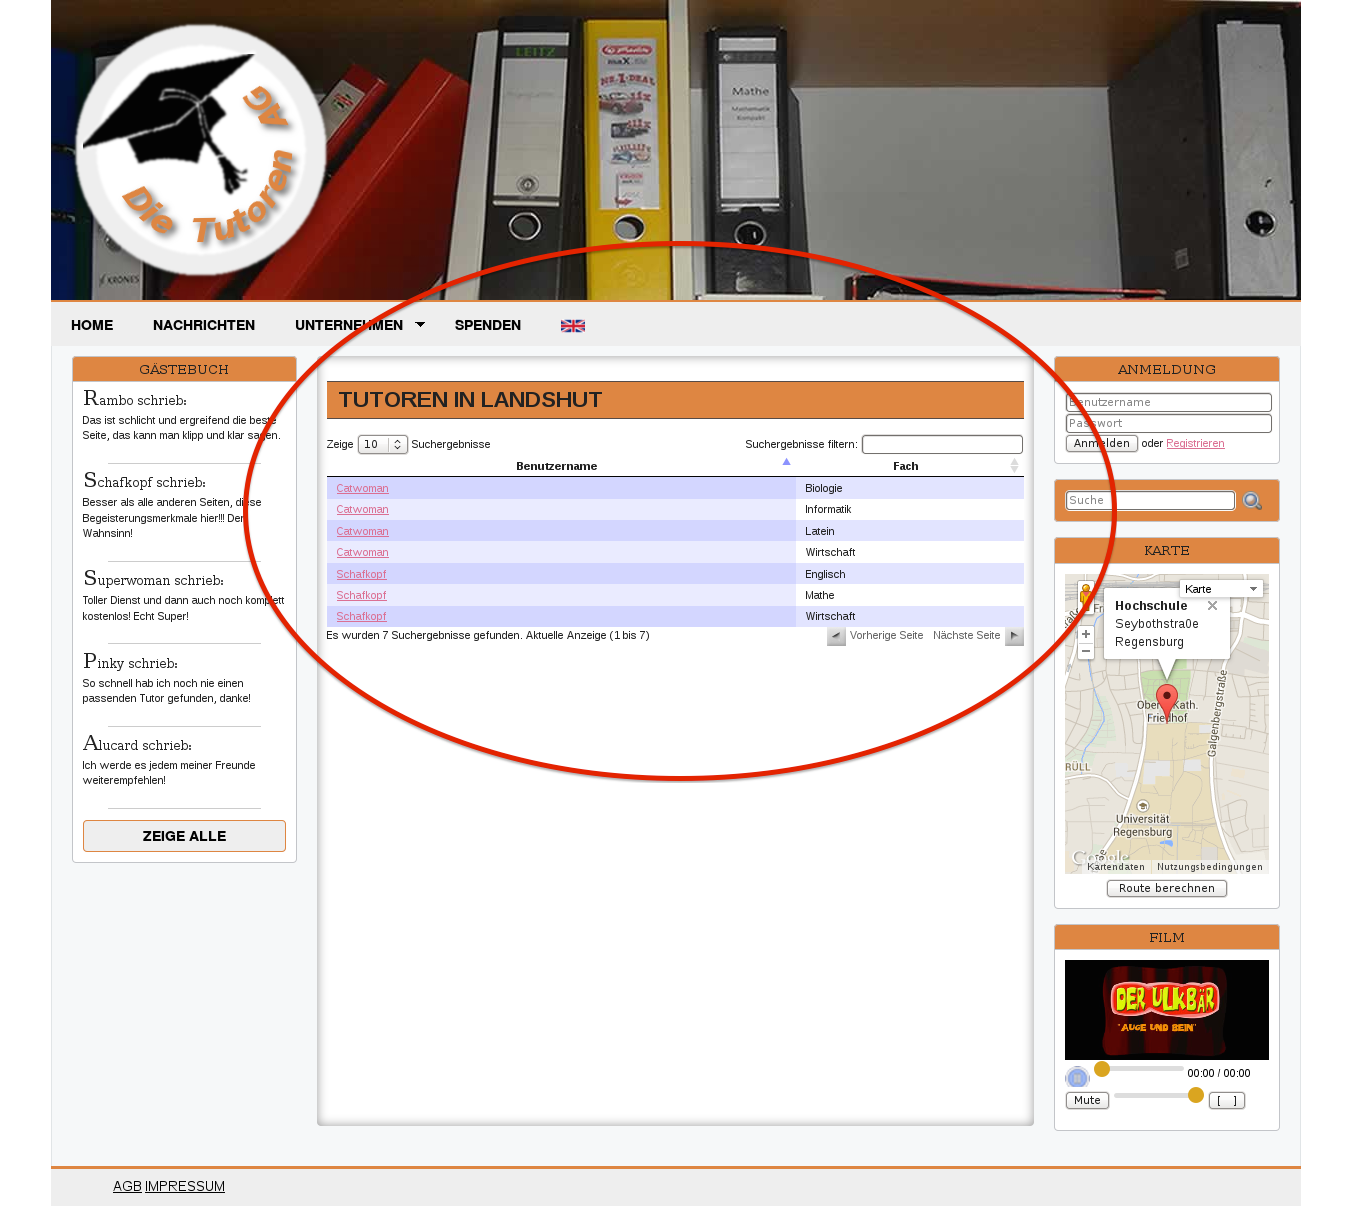
\includegraphics[width=1\linewidth]{../Screenshots/de/Suche_Ort}
\caption{Suchausgabe Wohnort}
\label{fig:SuchausgabeWohnort}
\end{figure}
